\section{Isomorphisms}
\begin{definition}
	Let $f:a\rightarrow b$ be an arrow in a category $\mathbb{C}$. An inverse for
	$f$ is an arrow $g:b\rightarrow a$ such that $g \circ f = 1_a$ and $f \circ g =
		1_b$.
\end{definition}

\begin{definition}
	Let $f:a\rightarrow b$ be an arrow in a category $\mathbb{C}$. If $f$ has an
	inverse we say that $f$ is invertible and call it an isomorphism, and we say
	that $a$ and $b$ are isomorphic. We use the notation $\cong$ as in $a \cong b$,
	or we write $a \xrightarrow{\sim} b$ .
\end{definition}

\subsection{Treating Isomorphisms as the Same}
\setcounter{tttacounter}{3}
\begin{ttta}
	Show that any object in a category is isomorphic to itself.
	\begin{proofitem}
		\item Suppose some object $a$. To show that $a$ is isomorphic to itself, we
		need some $g$ and $f$ such that $g\circ f=1_a$. Let $f=g=1_a$, and then
		$g\circ f=1_a \circ 1_a = 1_a$, and thus $a$ is isomorphic to itself.
	\end{proofitem}
\end{ttta}

\begin{ttta}
	Is it possible for an arrow to have two different inverses? It may help to think
	about the analogous question for additive inverses of numbers.
	\begin{proofitem}
		\item Let $f:a\rightarrow b$ and $g:b\rightarrow a$ be an arrow in category $\mathcal{C}$.
		\item Suppose $g_1$ and $g_2$ are both inverses for $f$. Then $g_1=g_2$. The
		proof is as follows
		\begin{align*}
			f\circ g_1 = 1_b     & = f\circ g_2           &  & \text{pre-compose }f    \\
			g_1\circ f = 1_a     & = g_2\circ f           &  & \text{post-compose }f   \\
			g_1 \circ f\circ g_1 & = g_1 \circ f\circ g_2 &  & \text{post-compose }g_1 \\
			1_a\circ g_1         & = 1_a \circ g_2                                     \\
			g_1                  & = g_2
		\end{align*}
	\end{proofitem}
	\begin{figure}[H]
		\begin{center}
			\documentclass{standalone}
\usepackage{tikz}
\begin{document}
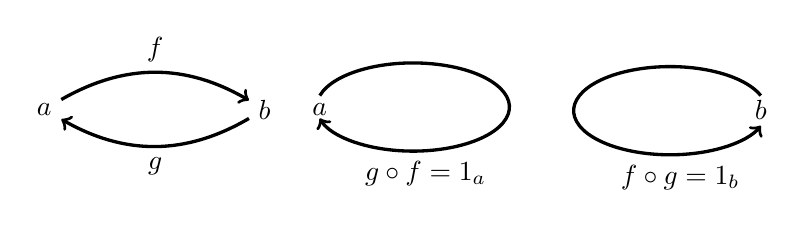
\begin{tikzpicture}[scale=0.7]
	\tikzset{arc lines/.style={very thick,black, ->}}
	% \draw (0, 0) grid (16, 2);

	\node (0) at (5, 0) {$a$};
	\node (1) at (5, 0.25) {};
	\draw[arc lines] (1) arc [start angle=15, end angle=345, x radius=-1.75cm, y
			radius=0.8cm]
	node[pos=0.75, below] {$g\circ f=1_a$}
	;
	\node (0) at (13, 0) {$b$};
	\node (1) at (13, 0.25) {};
	\draw[arc lines] (1) arc [start angle=20, end angle=340, x radius=1.75cm, y
			radius=0.8cm]
	node[pos=0.8, below] {$f\circ g=1_b$}
	;
	\node (0) at (0, 0) {$a$};
	\node (1) at (4, 0) {$b$};
	\draw [arc lines, ->, bend left=30] (0) to node[pos=0.5, above] {$f$} (1);
	\draw [arc lines, ->, bend left=30] (1) to node[pos=0.5, below] {$g$} (0);
\end{tikzpicture}
\end{document}

		\end{center}
		\caption{inverses and isomorphisms}
	\end{figure}
\end{ttta}

\stepcounter{tttacounter}
\begin{ttta}
	Show that $x$ has the same relationships with $a$ that it does with $b$.
	Consider a morphism $x\rightarrow a$ and use the isomorphism to produce a
	morphism $x\rightarrow b$. Then go back the other way.
\end{ttta}
\begin{figure}[H]
	\begin{center}
		\documentclass{standalone}
\usepackage{tikz}
\begin{document}
\begin{tikzpicture}[scale=0.7]
	\tikzset{arc lines/.style={very thick,black, ->}}
	% \draw (0, 0) grid (16, 2);
	\node (a) at (0, 0) {$a$};
	\node (b) at (4, 0) {$b$};
	\node (x) at (2, 4) {$x$};
	\draw[arc lines, dashed, ->] (x) to node[pos=0.5, left] {$s$} (0);
	\draw[arc lines, dashed, ->] (x) to node[pos=0.5, right] {$t$} (1);
	\draw [arc lines, ->, bend left=30] (a) to node[pos=0.5, above] {$f$} (b);
	\draw [arc lines, ->, bend left=30] (b) to node[pos=0.5, below] {$g$} (a);
\end{tikzpicture}
\end{document}

	\end{center}
	\caption{inverses and isomorphisms}
\end{figure}
\subsubsection{Example}
\begin{proofitem}
	\item Let $X=\set{S, M}$, $A=\set{1, 2, 3}$, $B=\set{a, b, c}$.
\end{proofitem}

\begin{proofitem}
	\item Let $f:a\rightarrow b$, $g:b\rightarrow a$, and $f$ and $g$ are inverses,
	and therefore $a$ and $b$ are isomorphic.
	\item
	Since any morphism $s: x \rightarrow a$ can be recovered by composing the
	corresponding morphism $t = f \circ s : x \rightarrow b$ with the inverse
	$g$ of the isomorphism $f$, it shows that every relationship between $x$ and
	a can be translated into an equivalent relationship between $x$ and $b$
	using the isomorphism.
	\item Same idea for $t: x\rightarrow b$.
	\setcounter{equation}{0}
	\begin{align}
		s                  &  & x\rightarrow a \\
		f\circ s = t       &  & x\rightarrow b \\
		g\circ f\circ s= s &  & x\rightarrow a \\
		t                  &  & x\rightarrow b \\
		t\circ g = s                           \\
		f\circ g\circ t= t
	\end{align}
	Note that we went from (1) to (2) to (3), and showed that (1) and (3) are
	equivalent. Therefore (2) is also equivalent. We can use the same logic for (4)
	- (6).
\end{proofitem}

\begin{ttta}
	Show that $x$ has the same relationships with $a$ that it does with $b$.
	Consider a morphism $s: a\rightarrow x$ and use the isomorphism to produce a
	morphism $t: b\rightarrow x$. Then go back the other way.
\end{ttta}
\begin{proofitem}
	\item Let $f:a\rightarrow b$, $g:b\rightarrow a$, and $f$ and $g$ are inverses,
	and therefore $a$ and $b$ are isomorphic.
	\item
	Since any morphism $s: a \rightarrow x$ can be recovered by composing the
	corresponding morphism $s \circ g : b \rightarrow x$ with the inverse
	$f$ of the isomorphism $g$, it shows that every relationship between $a$ and
	$x$ can be translated into an equivalent relationship between $b$ and $x$
	using the isomorphism.
\end{proofitem}
\setcounter{equation}{0}
\begin{align}
	s                    &  & a\rightarrow x \\
	s\circ g             &  & b\rightarrow x \\
	s\circ g \circ f = s &  & a\rightarrow x \\
	t                    &  & b\rightarrow x \\
	t\circ f             &  & a\rightarrow x \\
	t\circ f \circ g = t &  & b\rightarrow x
\end{align}
\begin{figure}[H]
	\begin{center}
		\documentclass{standalone}
\usepackage{tikz}
\begin{document}
\begin{tikzpicture}[scale=0.7]
    \tikzset{arc lines/.style={very thick,black, ->}}
    \node (a) at (0, 0) {$a$};
    \node (b) at (4, 0) {$b$};
    \node (x) at (2, 4) {$x$};
    \draw[arc lines, dashed, ->] (0) to node[pos=0.5, left] {$s$} (x);
    \draw[arc lines, dashed, ->] (1) to node[pos=0.5, right] {$t$} (x);
    \draw [arc lines, ->, bend left=30] (a) to node[pos=0.5, above] {$f$} (b);
    \draw [arc lines, ->, bend left=30] (b) to node[pos=0.5, below] {$g$} (a);
\end{tikzpicture}
\end{document}

	\end{center}
	\caption{inverses and isomorphisms}
\end{figure}

\subsection{Isomorphisms of Sets}
\begin{ttta}
	1. Take $A = {a, b, c}$ and $B = {1, 2, 3}$. Can you construct an isomorphism
	between them? How many different ones are there?
	2. Now take $A = {a, b, c}$ and $B = {1, 2}$. Why is it not possible to
	construct an isomorphism?
	3. Can you come up with a theory of when it is and isn’t possible to construct
	an isomorphism between sets?
\end{ttta}
\begin{proofitem}
	\item For $A$ and $B$ to be isomorphic, there must exist an invertible function
	$f: A\rightarrow B$ such that $f\circ f^{-1} = 1_B$ and $f^{-1}\circ f=1_A$.
	\item One possibility for $f$ is the relation $f\subseteq A\times B=\set{(a, 1),
			(b, 2), (c, 3)}$ and $f^{-1}\subseteq B\times A=\set{(1, a), (2, b), (3,
			c)}$.
	\begin{align*}
		(f^{-1}\circ f)(a) = f^{-1}(f(a)) = f^{-1}(1) = a \\
		(f^{-1}\circ f)(b) = f^{-1}(f(b)) = f^{-1}(2) = b \\
		(f^{-1}\circ f)(c) = f^{-1}(f(c)) = f^{-1}(3) = c
	\end{align*}
	\item It is not possible to create an isomorphism between $A$ and $B$ when
	$|A|\neq|B|$. An isomorphism between sets is the same as a bijective
	function, and bijection is only possible with sets of equal cardinality.
\end{proofitem}
\clearpage

\begin{ttta}
	Prove that a function is an isomorphism of sets if and only if it is a bijection.
\end{ttta}
\begin{proofitem}
	\item Proof of $\text{isomorphism}\implies \text{bijection}$:
	\begin{proofitem}
		\item Because $A$ and $B$ are isomorphic, there exists an invertible function
		$f$ such that $f\circ f^{-1}=1_b$ and $f^{-1}\circ f = 1_a$.
		\item Suppose $a_1 \land a_2 \in A$ such that $f(a_1)=f(a_2)$.
		\begin{align*}
			f(a_1) =               & f(a_2)                                           \\
			f^{-1}(f(a_1)) =       & f^{-1}(f(a_2))       &  & \text{apply inverse}   \\
			(f^{-1}\circ f)(a_1) = & (f^{-1}\circ f)(a_2) &  & \text{def. of }\circ   \\
			1_a(a_1) =             & 1_a(a_2)             &  & \text{via isomorphism} \\
			a_1 =                  & a_2
		\end{align*}
		Thus we have shown via the converse implication of injection, that if $f(a_1)=f(a_2)$, then $a_1=a_2$ by
		using the isomorphism between $A$ and $B$.
		\item Suppose some $b\in B$.
		\begin{align*}
			f(a) =               & b                                     \\
			f^{-1}(f(a)) =       & f^{-1}(b) &  & \text{apply inverse}   \\
			(f^{-1}\circ f)(a) = & f^{-1}(b) &  & \text{def. of }\circ   \\
			1_a(a) =             & f^{-1}(b) &  & \text{via isomorphism} \\
			a =                  & f^{-1}(b)
		\end{align*}
		Therefore we have shown that for some arbitrary $b\in B$. we can produce an
		$a\in A$ such that that $f(a)=b$ by applying $f^{-1}$ to $b$. Thus we have shown
		that $f$ is injective and surjective if $f$ is isomorphic, and therefore $f$ is
		bijective if $f$ is isomorphic.
	\end{proofitem}
	\item Proof of $\text{bijection}\implies \text{isomorphism}$:
	\begin{proofitem}
		\item Since $f$ is bijective, an inverse $f^{-1}$ exists. By definition of
		inverse, there exists a composition $f\circ f^{-1}=1_b$ and $f^{-1}\circ
			f=1_a$.
	\end{proofitem}
	Therefore we have proved the implication both ways, and shown that a function is
	an isomorphism of sets if and only if it is a bijection.
\end{proofitem}

\subsection{Isomorphism of Large Structures}
\begin{ttta}
	Can you show that a morphism $f:A\rightarrow B$ of monoids is an isomorphism in the
	category of monoids if and only if it is a bijective homomorphism?
\end{ttta}
The content of this is that we don’t have to insist on the inverse being
structure-preserving because it will automatically follow.

\begin{proofitem}
	\item Proof of $\text{bijective homomorphism}\implies \text{isomorphism in
		}\mathcal{C}$:
	\item Suppose $f:A\rightarrow B$ is a bijective homomorphism.
	\begin{align*}
		f(X\circ Y) =                & f(X) \circ f(Y)         &  & \text{homomorphism} \\
		f^{-1}(f(X\circ Y)) =        & f^{-1}(f(X) \circ f(Y)) &  & \text{bijection}    \\
		(f^{-1}\times f)(X\circ Y) = & f^{-1}(f(X) \circ f(Y))                          \\
		X\circ Y =                   & f^{-1}(f(X) \circ f(Y))
	\end{align*}
	\item
	Therefore we have shown that the composition of monoidal elements
	$f(X) \circ f(Y)$ has an inverse, and therefore is an an isomorphism.
\end{proofitem}
\begin{proofitem}
	\item
	Proof of $ \text{isomorphism in }\mathcal{C} \implies \text{bijective
			homomorphism} $:
	\begin{align*}
		X\circ Y = & (f\times f^{-1})(X\circ Y) &  & \text{isomorphism} \\
		=          & f(f^{-1}(X\circ Y))
	\end{align*}
	\item
\end{proofitem}

% \addtocounter{tttacounter}{-1}
% \begin{ttta}
% Can you show the analogous result is true for posets?
% \end{ttta}

% \addtocounter{tttacounter}{-1}
% \begin{ttta}
% Can you show that the analogous result for topological spaces is not true?
% \end{ttta}
% \begin{proofitem}
% \end{proofitem}
